\chapter{Simulation: Uniform Scenarios}
\section{Introduction}
In this chapter we will consider \texttt{Mobile Stations} which, at each timeslot, generate CQIs with an integer uniform distribution. In the validation scenario we proved that scheduler is fair so we expect that all users will have similar values for the mean throughput and the mean response time. In this simulation we will consider the following parameters:
\begin{itemize}
	\item \(n=10\)
	\item \(packetsize_{i} \sim U(3,75), \quad 0 \le i \le n-1\)
	\item \(CQI_{i} \sim U(1,15), \quad 0 \le i \le n-1\)
	\item \( \lambda = \lambda_{i} = 0.1 + 0.5k, \quad k\in\{1,2\ldots,10\}, \quad 0 \le i \le n-1\)
\end{itemize}
This scenario is almost similar to the NoFraming Validation test, but the main difference is that \(packetsize\) is a uniform RV. As we said before we expect to get worse throughput result due to the fact that some RB space will be left empty because packets cannot be fragmented. 

We will simulate the scenario with both scheduler and we will check if our first intuition is true or not and the impact of \textbf{framing} in the average performance metrics.

\section{Uniform CQI, Fair Scheduler}
In this simulation we will consider the basic \textbf{Fair Scheduler}. We remember that, in this case, if \(currentUser\) empties his queue or has a packet that is bigger than \(RB_{size}\) the scheduler will consider the next users.

\begin{figure}[H]
  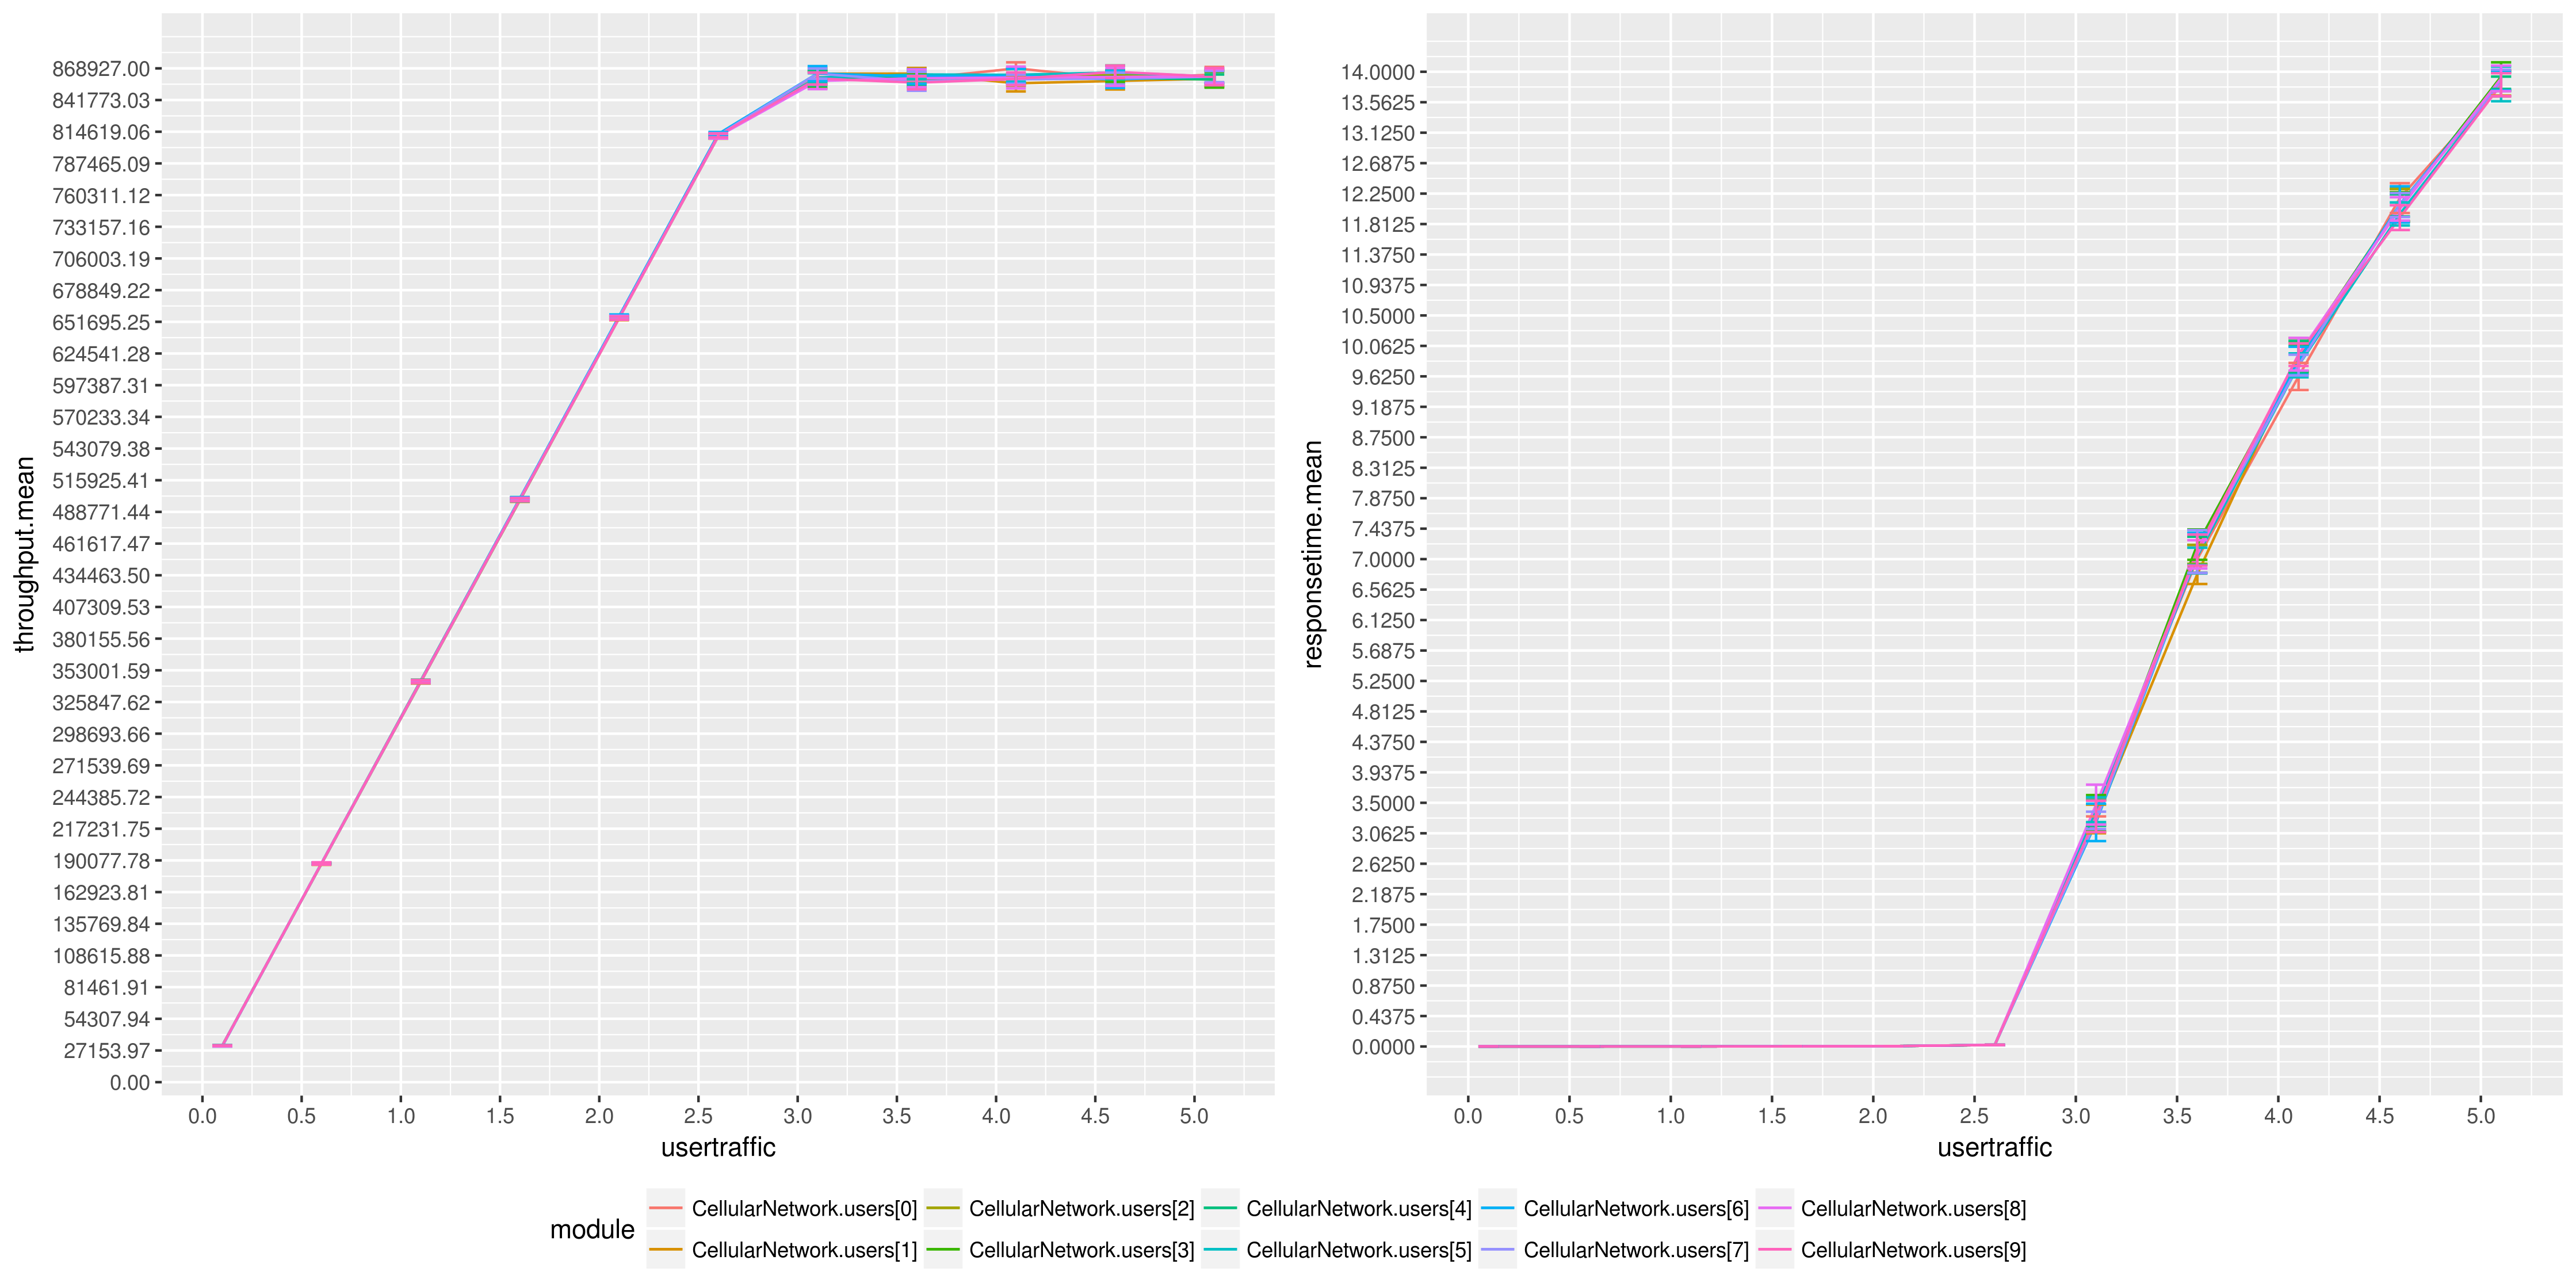
\includegraphics[width=1\textwidth]{images/unif}
  \caption{Uniform scenario - Fair: throughput, response time}
  \label{fig:Uniform scenario - Fair: throughput, response time}
\end{figure}
The first thing we can notice is that every client has the same saturation point (which depends on \(\lambda\)): this can be explained considering that scheduler is fair and every client generates, on average, the same amount of packets (which are also the same size on average). Response times are stable before reaching the common saturation point and after tends to arise indefinitely, until reaching a maximum. This maximum is the same shown in the \(2_{nd}\) Validation test and has the same explaination. So the only valid values for Response Times are generated between \(0 < \lambda < \lambda_{sat}\), which is common for each client. 

In the graph we notice that \(\lambda_{sat}=3.1\). If we compare this rate with the maximum rate computed in the 1\textsuperscript{st} Validation Test we observe that \(\lambda_{sat} = \lambda_{max}/10\). This is not surprising since there are 10 \texttt{Web Server} wich push traffic to the Antenna. Each one is a \textit{Poisson process} with rate \(\lambda\) so the superimposition of 10 them is a \textit{Poisson process} with a rate \(\Lambda = 10\lambda\). Actually the system saturates before \(\lambda=3.1\), infact in validation we considered the best case where \(CQI=15\) so RBs had the maximum size. Here \(RB_{size}\) is a RV however \(\lambda_{sat}=3.1\) is a raw approximation confirmed by the results of the simulation.

The most important result, here, is the antenna total throughput. Lets see:
\begin{figure}[H]
  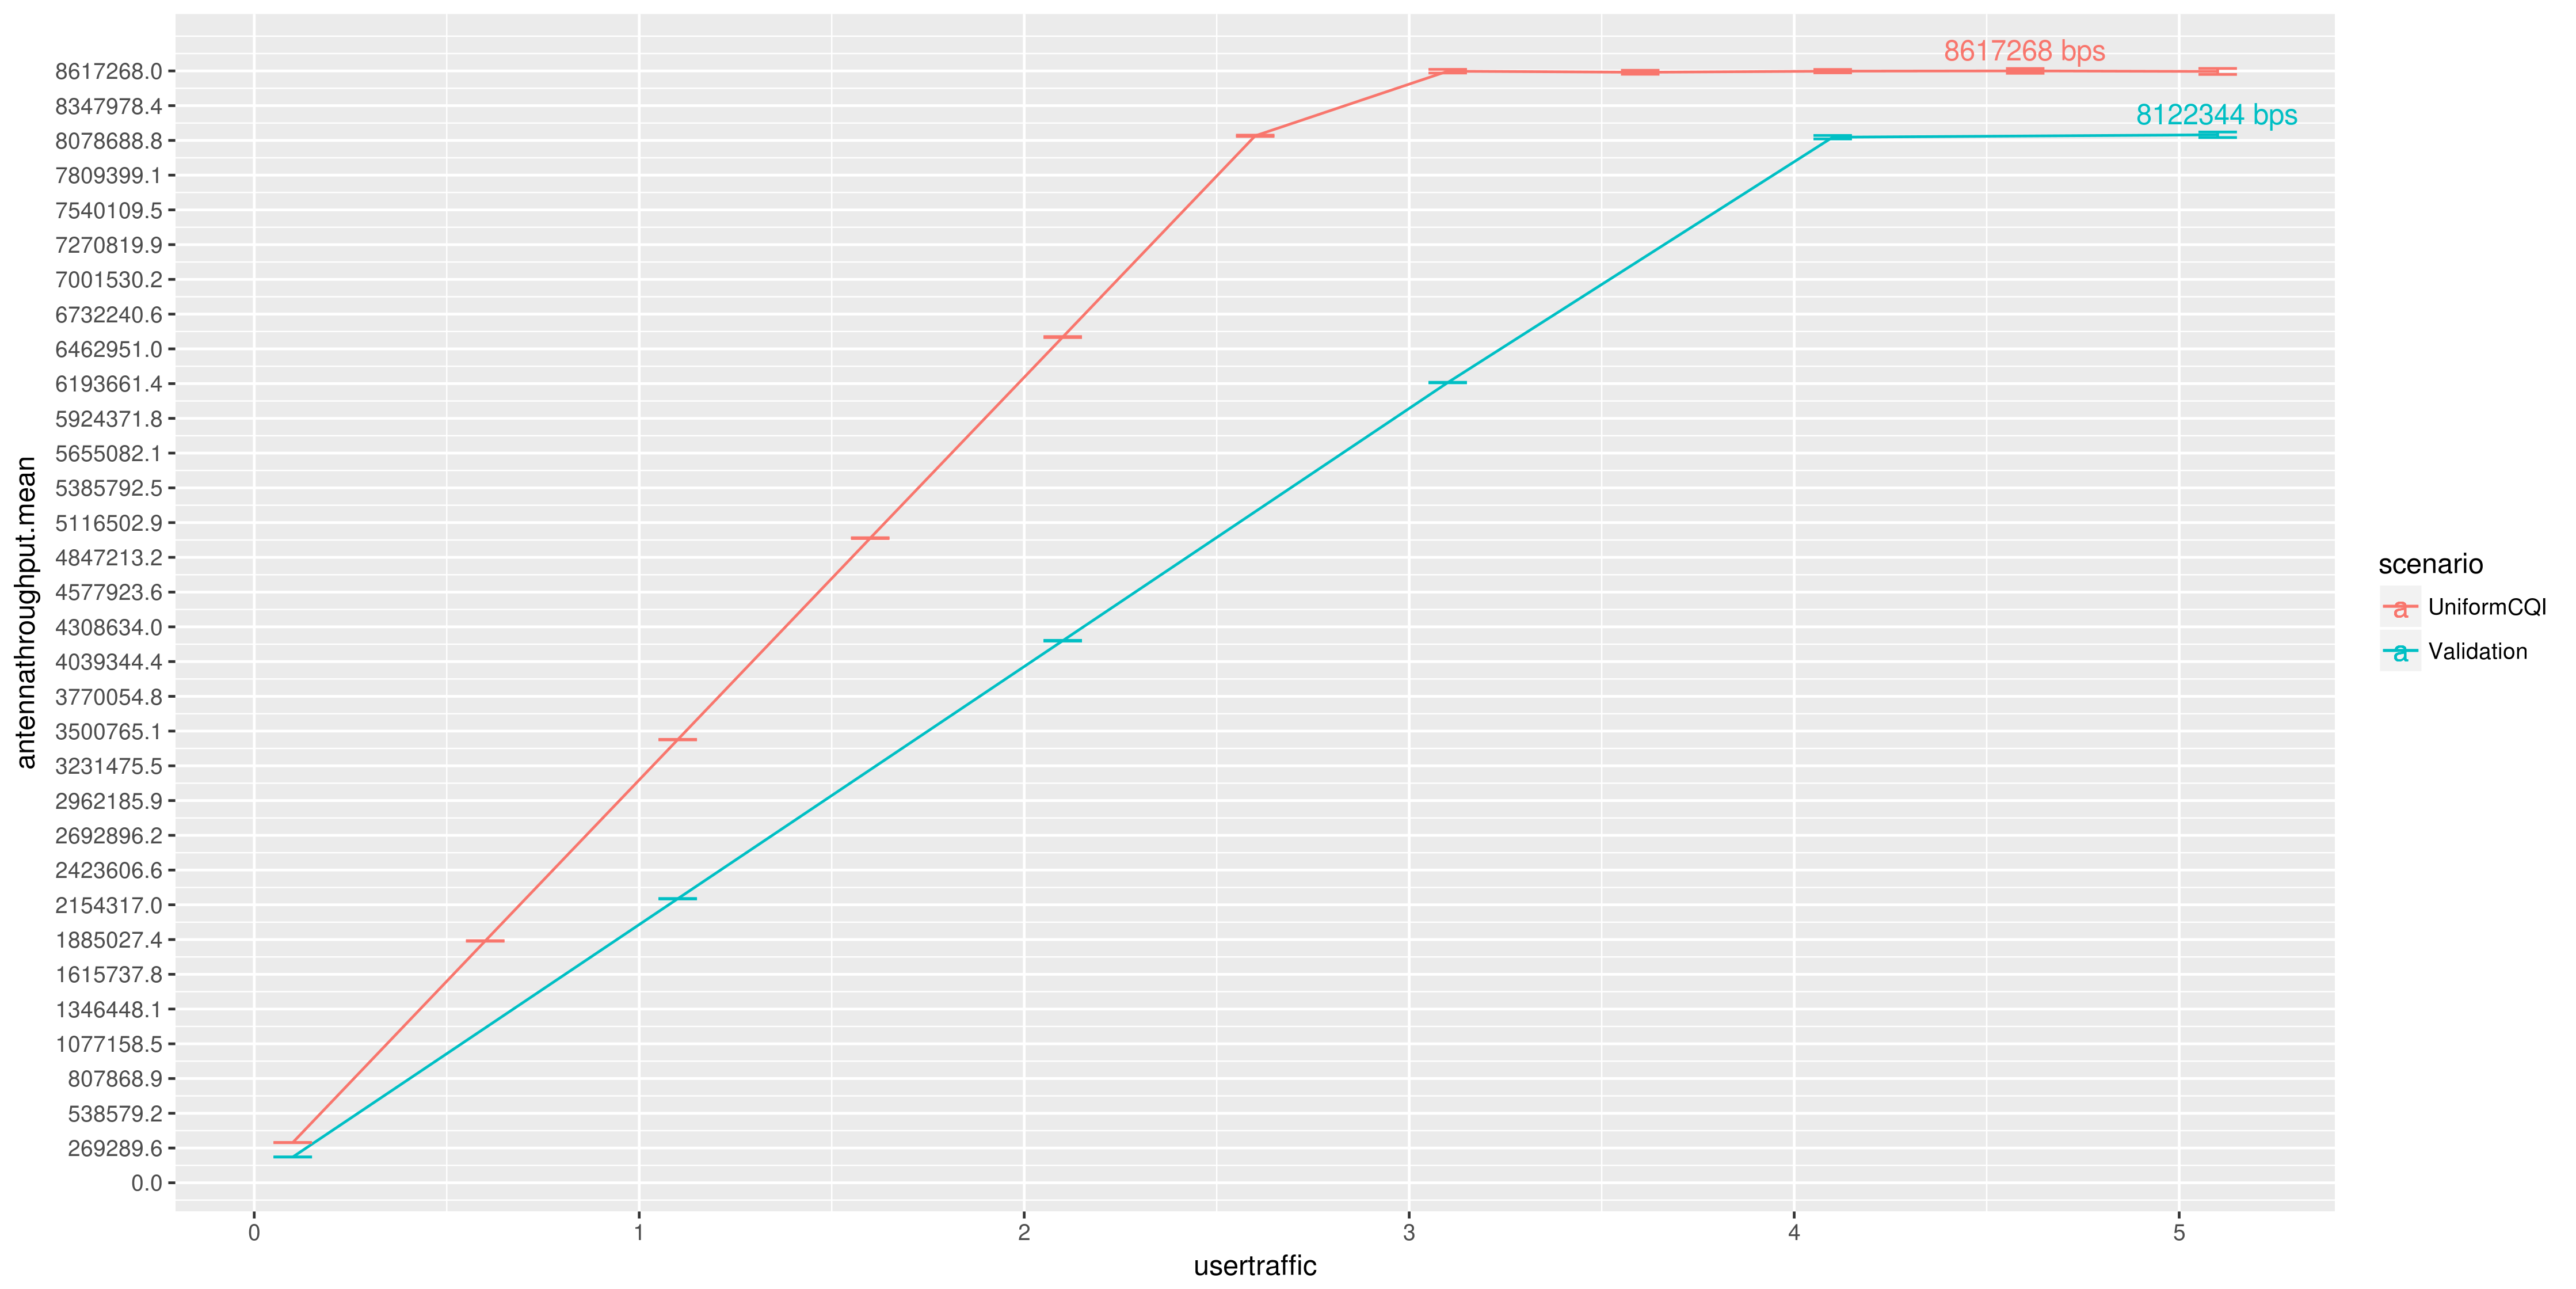
\includegraphics[width=1\textwidth]{images/thantenna1}
  \caption{Antenna throughput: UniformCQI, Validation-NoFramingTest}
  \label{fig:Antenna throughput: UniformCQI, Validation-NoFramingTest}
\end{figure}

Comparing to the 3\textsuperscript{rd} NoFraming Validation test result, our global throughput is \textbf{higher}. This is a very very strange result that \textbf{destroys our first intuition} about the impact of framing.

How can the throughput get higher? Thinking about our model, we came up with a possible explanation. Framing policies, as we seen before, are basically two:
\begin{itemize}
	\item One RB cannot contain traffic from 2 or more different clients
	\item If a packet cannot entirely fit the frame, it cannot be scheduled
\end{itemize}
The first policy cannot give us an higher throughput and this is already proven: we are telling that some frame space is eventually wasted, and this leads always to a worse or equal throughput result. So lets focus on the second policy: our intuition (hopefully correct this time) suggests us that framing, as a measure of how much RBs are not filled due to framing, is uniformly distributed for each client. Lets remember that the remaining space is allocated to other clients using a Fair policy (FairScheduler) and \(framesize_i\) depends on \(rbsize_i = f(CQI_i)\). Now lets try to analyze a single iteration of the scheduler algorithm, applied to 2 clients in the following state:
\begin{align}
 \#RB_{free} &= 1, &currentUser &= 1 \nonumber \\
 	   CQI_1 &= 1, &rbsize_1 &= 3 \nonumber \\
	   CQI_2 &= 13, &rbsize_2 &= 80 \nonumber
\end{align}

Both have one packet of \(packetsize=75\) (which is the maximum we can have) in backlog. The first client cannot fit his packet into the frame chunk, so remaining RBs (in our case just 1) are allocated to the client 2, which can now fit his packet into his frame chunk. The main factor, here, is \(framechunksize_i = remainingRBfor_i \times rbsize_i\): we are telling that client with the best CQI can fit more likely his packets into the frame, despite of the current serving user, due to the fact that his \(framechunksize_i\) is bigger than the other clients. This reminds us a bit of BestCQI Scheduler policies.

However we must consider that the previous case does not describe completely all the possible behaviors of the system. Infact, lets consider this other case:
\begin{align}
	\#RB_{free} &= 1, &currentUser &= 1 \nonumber \\ 
	CQI_1 &= 3, &rbsize_1 &= 6, & backlog &= \textnormal{1 packet of 75 bytes} \nonumber \\
	CQI_2 &= 1, &rbsize_2 &= 3, &backlog &= \textnormal{1 packet of 3 bytes} \nonumber \\
	CQI_3 &= 13, &rbsize_3 &= 80, &backlog &= \textnormal{1 packet of 75 bytes} \nonumber 
\end{align}

Client 1 packet cannot be scheduled (\(75 > 6\)), so we go next to the second user which can now fit his packet into the new frame chunk (3 = 3). As we can see here, the RB is allocated to the user with the worst CQI (client 2) and not the best (client 3). So we can also deduce that a client with a small packet in backlog is more likely to fit his packet into the frame.

Combining this result with the previous we can infer that a packet is more likely to fit if:
\begin{itemize}
	\item The packet is small
	\item The user CQI is high
\end{itemize}
We can add another case:
\begin{align}
	\#RB_{free} &= 1, &currentUser &= 1 \nonumber \\
	CQI_1 &= 3, &rbsize_1 &= 6, &backlog &= \textnormal{1 packet of 75 bytes} \nonumber\\
	CQI_2 &= 1, &rbsize_2 &= 3, &backlog &= \textnormal{1 packet of 75 bytes} \nonumber\\
	CQI_3 &= 2, &rbsize_3 &= 3, &backlog &= \textnormal{1 packet of 75 bytes} \nonumber
\end{align}
None of the packets cannot be inserted into the framechunk, so the RB is completely wasted. This is the case that lowers the throughput, due to the fact that packet sizes are small and CQIs are low. However, in our scenarios (Uniform, UniformBest, Binomial ...) the number of users is high enough (10 users) to get, more likely, at least a small packet and/or at least a good enough CQIs to not waste the remaining space.

%At the end we can see that this result lies between \textit{NoFramingTest} and \textit{Uniform BestCQI} results: in fact ``The user CQI is high'' is the main policy of BestCQI scheduler. However, in that scenario, we can't consider ``The packet is small'' because BestCQI user is \textbf{always} selected as first for the residual frame filling, and this increases the throughput for BestCQI scenario.

%CQIs and packet sizes are always uniform for all clients, so we suspect that all clients will benefit of a small and equal throughput increase.
%\begin{center}
%	INSERIRE IMMAGINE QUI ALLTH NOFRAMINGTEST EVENTUALMENTE, magari confrontare il test con quelli dell'uniform e far vedere che i throughput sono più bassi in NoFrameFilling
%\end{center}
%\

Note that we have tried to analyze just few cases and do a very raw approximation of antenna total throughput mean value tendency, so we can't make an exact model of the system in order to proof this result analytically. 
At the end of simulation we can summarize these results about the Uniform Scenario with Fair Scheduler:
\begin{itemize}
	\item Saturation rate \(\lambda = 3.1\)
	\item Antenna throughput \(th_{antenna} = 8615055 \pm 14206 \textnormal{ bps}\), \textit{conf lvl 95\%}
	\item User throughput \(th_{i} = 861343 \pm 4968 \textnormal{ bps}\), \textit{conf lvl 95\%}
\end{itemize} 

\section{Uniform, Best CQI scheduler}
Now we will simulate the scenario by using the second scheduler. If there were not \textbf{framing} the performance of both scheduler would be the same but, as seen before, \textbf{framing} is present and has a great impact in performance. We can expect this scheduler will have better performance in throughput since it fills the residual space inside the frame by using packets addressed to users with higher CQIs.
\begin{figure}[H]
  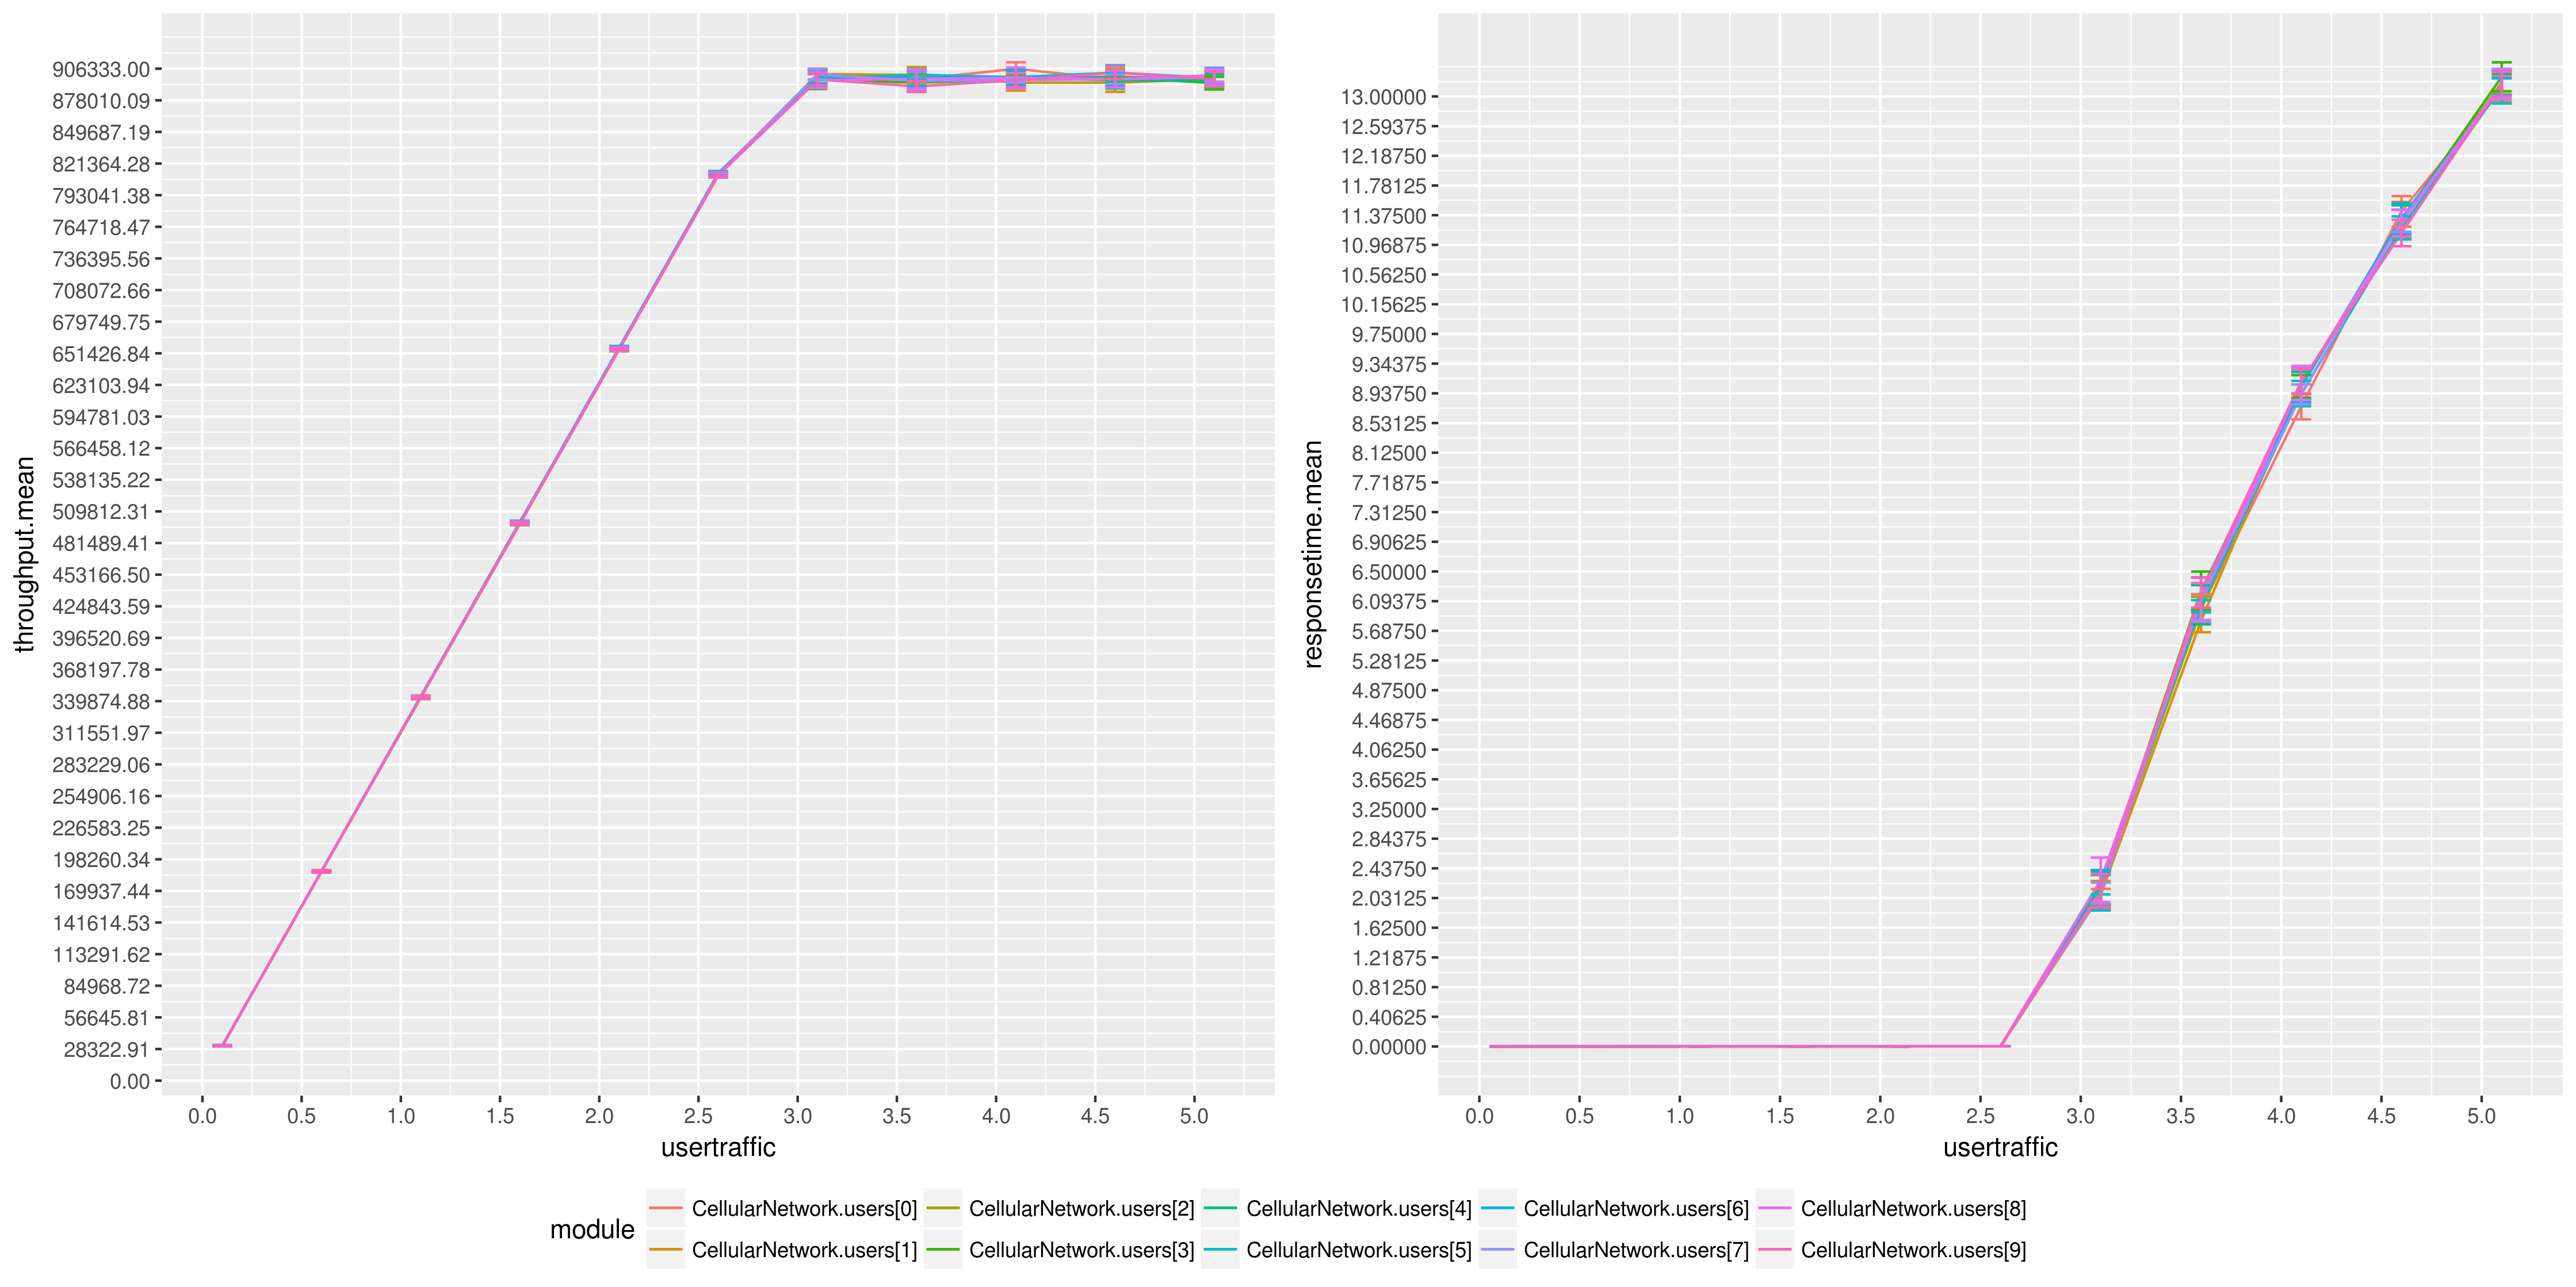
\includegraphics[width=1\textwidth]{images/unifbest}
   \caption{Uniform scenario - BestCQI: throughput, response time}
  \label{fig:Uniform scenario - BestCQI: throughput, response time}
\end{figure}

Result for Uniform Scenario with Best CQI Scheduler in saturation:
\begin{itemize}
	\item Saturation rate \(\lambda = 3.1\)
	\item Antenna throughput \(th_{antenna} = 8981747 \pm 14355 \textnormal{ bps}\), \textit{conf lvl 95\%}
	\item User throughput \(th_{i} = 897148 \pm 4772 \textnormal{ bps}\), \textit{conf lvl 95\%}
\end{itemize} 
We can see cleary an increase of throughput per each user and smaller the response time with respect to fair scheduler. The saturation point is the same at about \(\lambda=3.1\) but the throughput as we said is higher. The reason is that the residual space in the frame is used better since it is selected the user with the best CQI in order to carry as much data as possible. We can see also that the throughput distribution is fair among the users if we plot the lorenz curves for throughput and response time.
\begin{figure}[H]
\begin{minipage}[b]{8cm}
	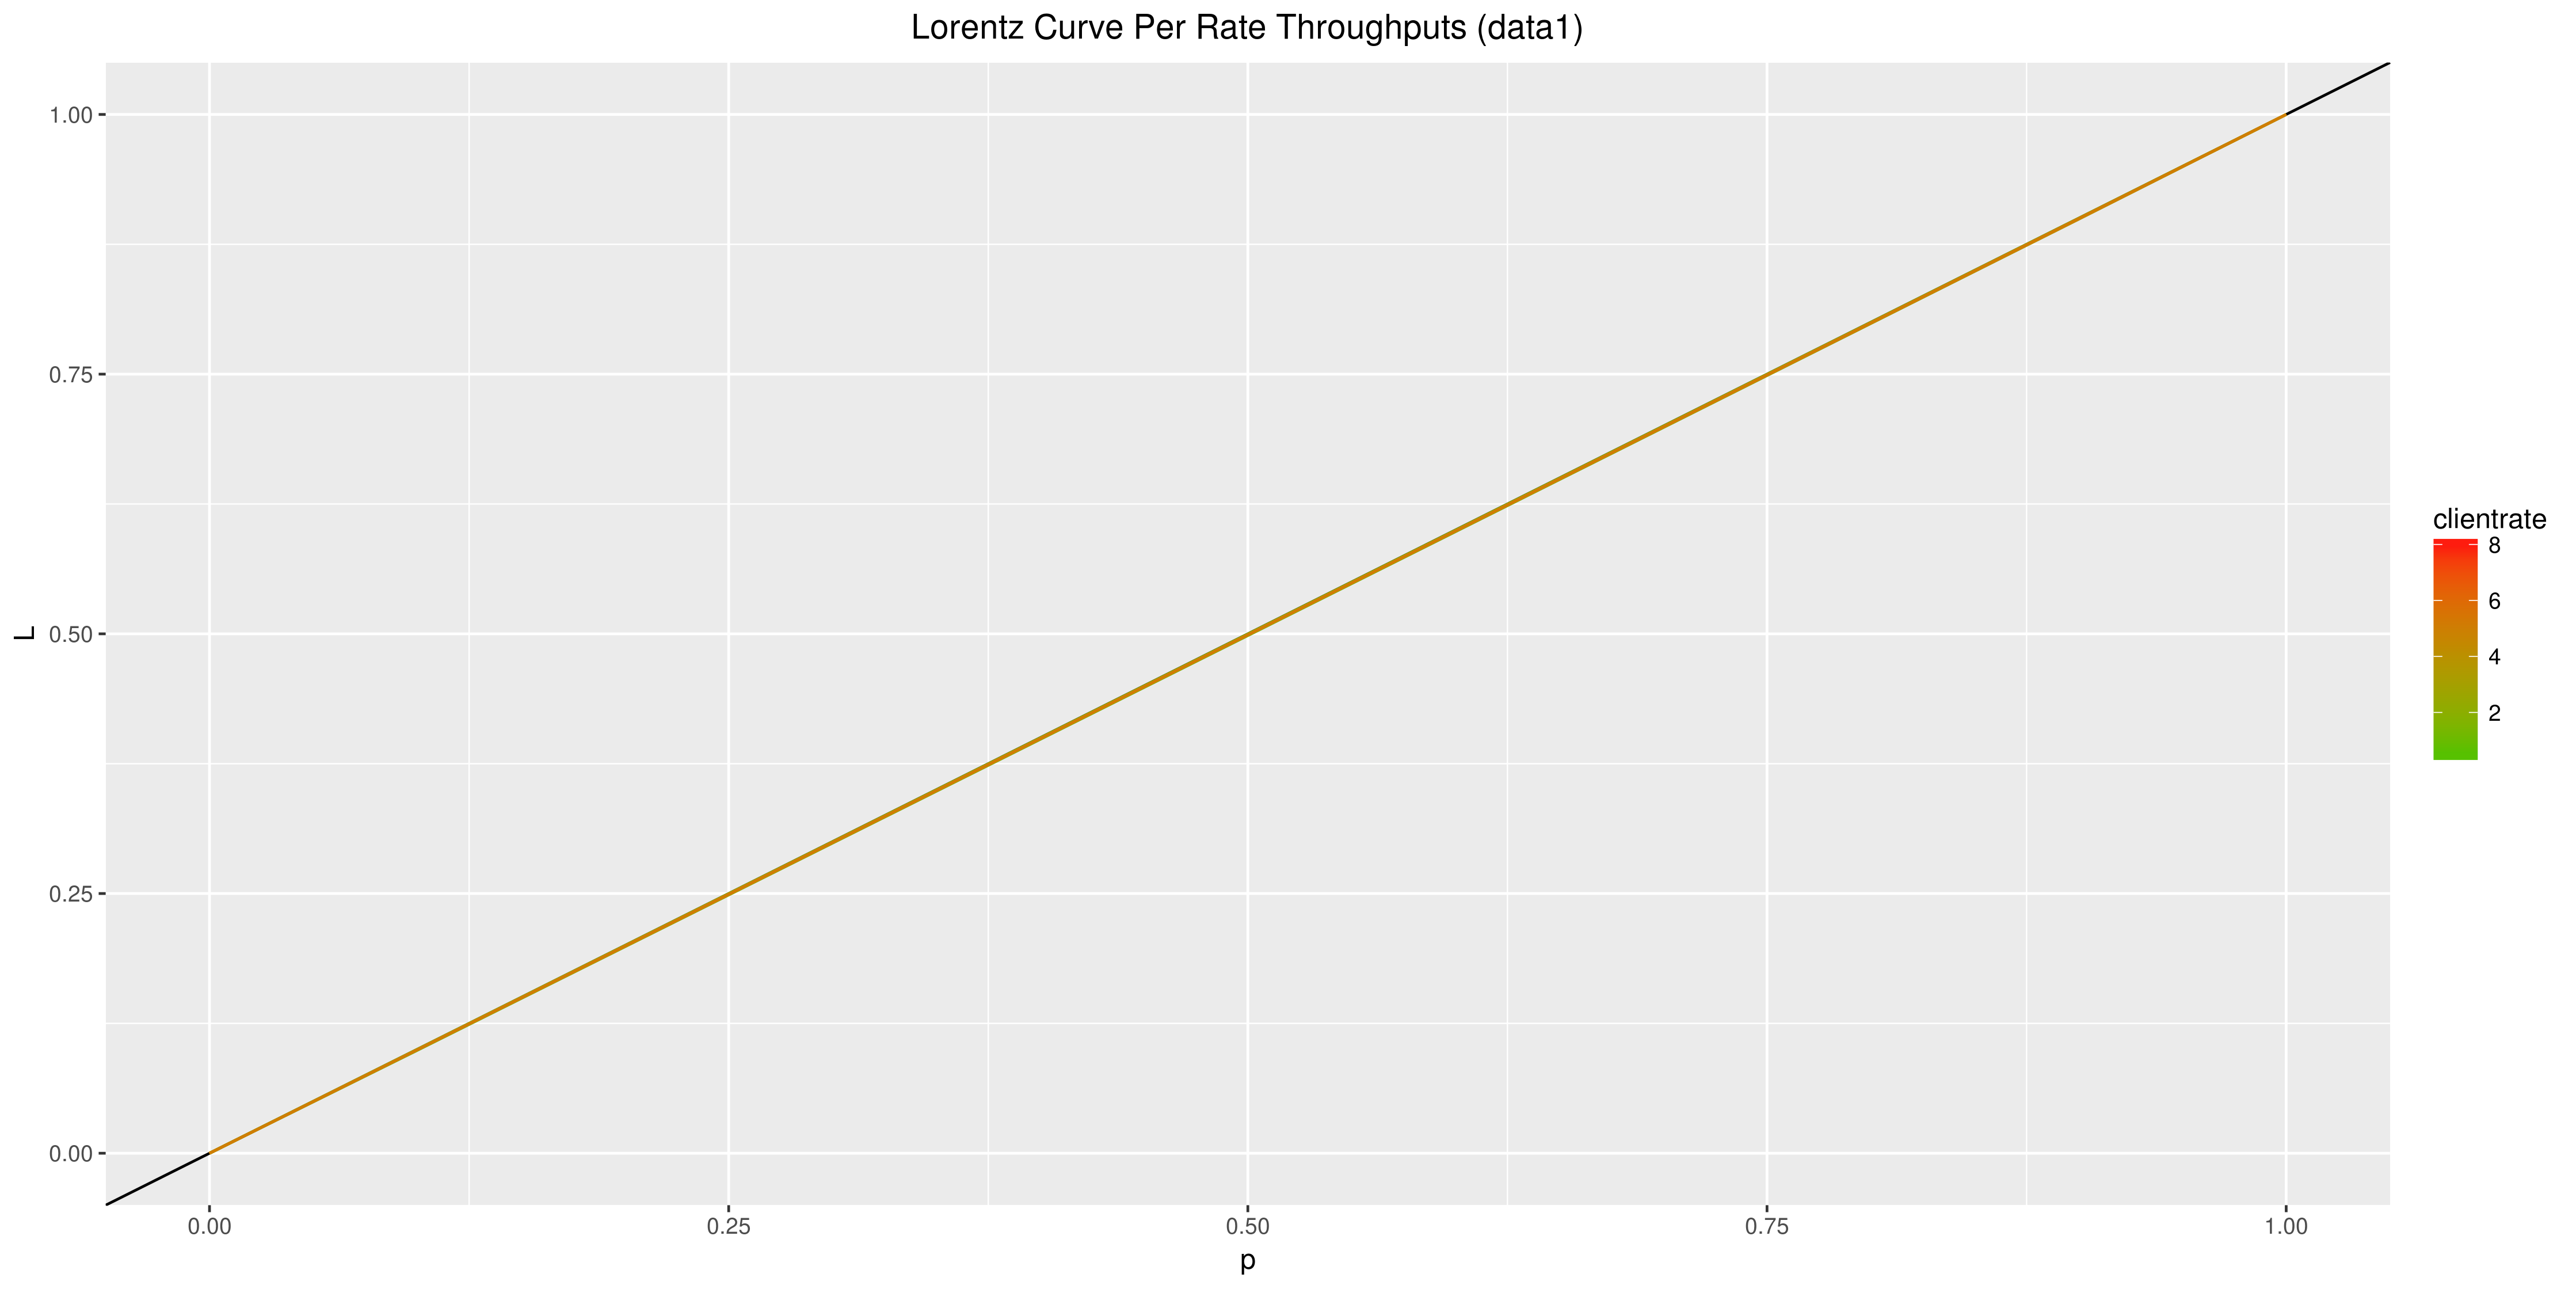
\includegraphics[width=7.5cm]{images/lorenzTH-unifbest}
\end{minipage}
\begin{minipage}[b]{8cm}
	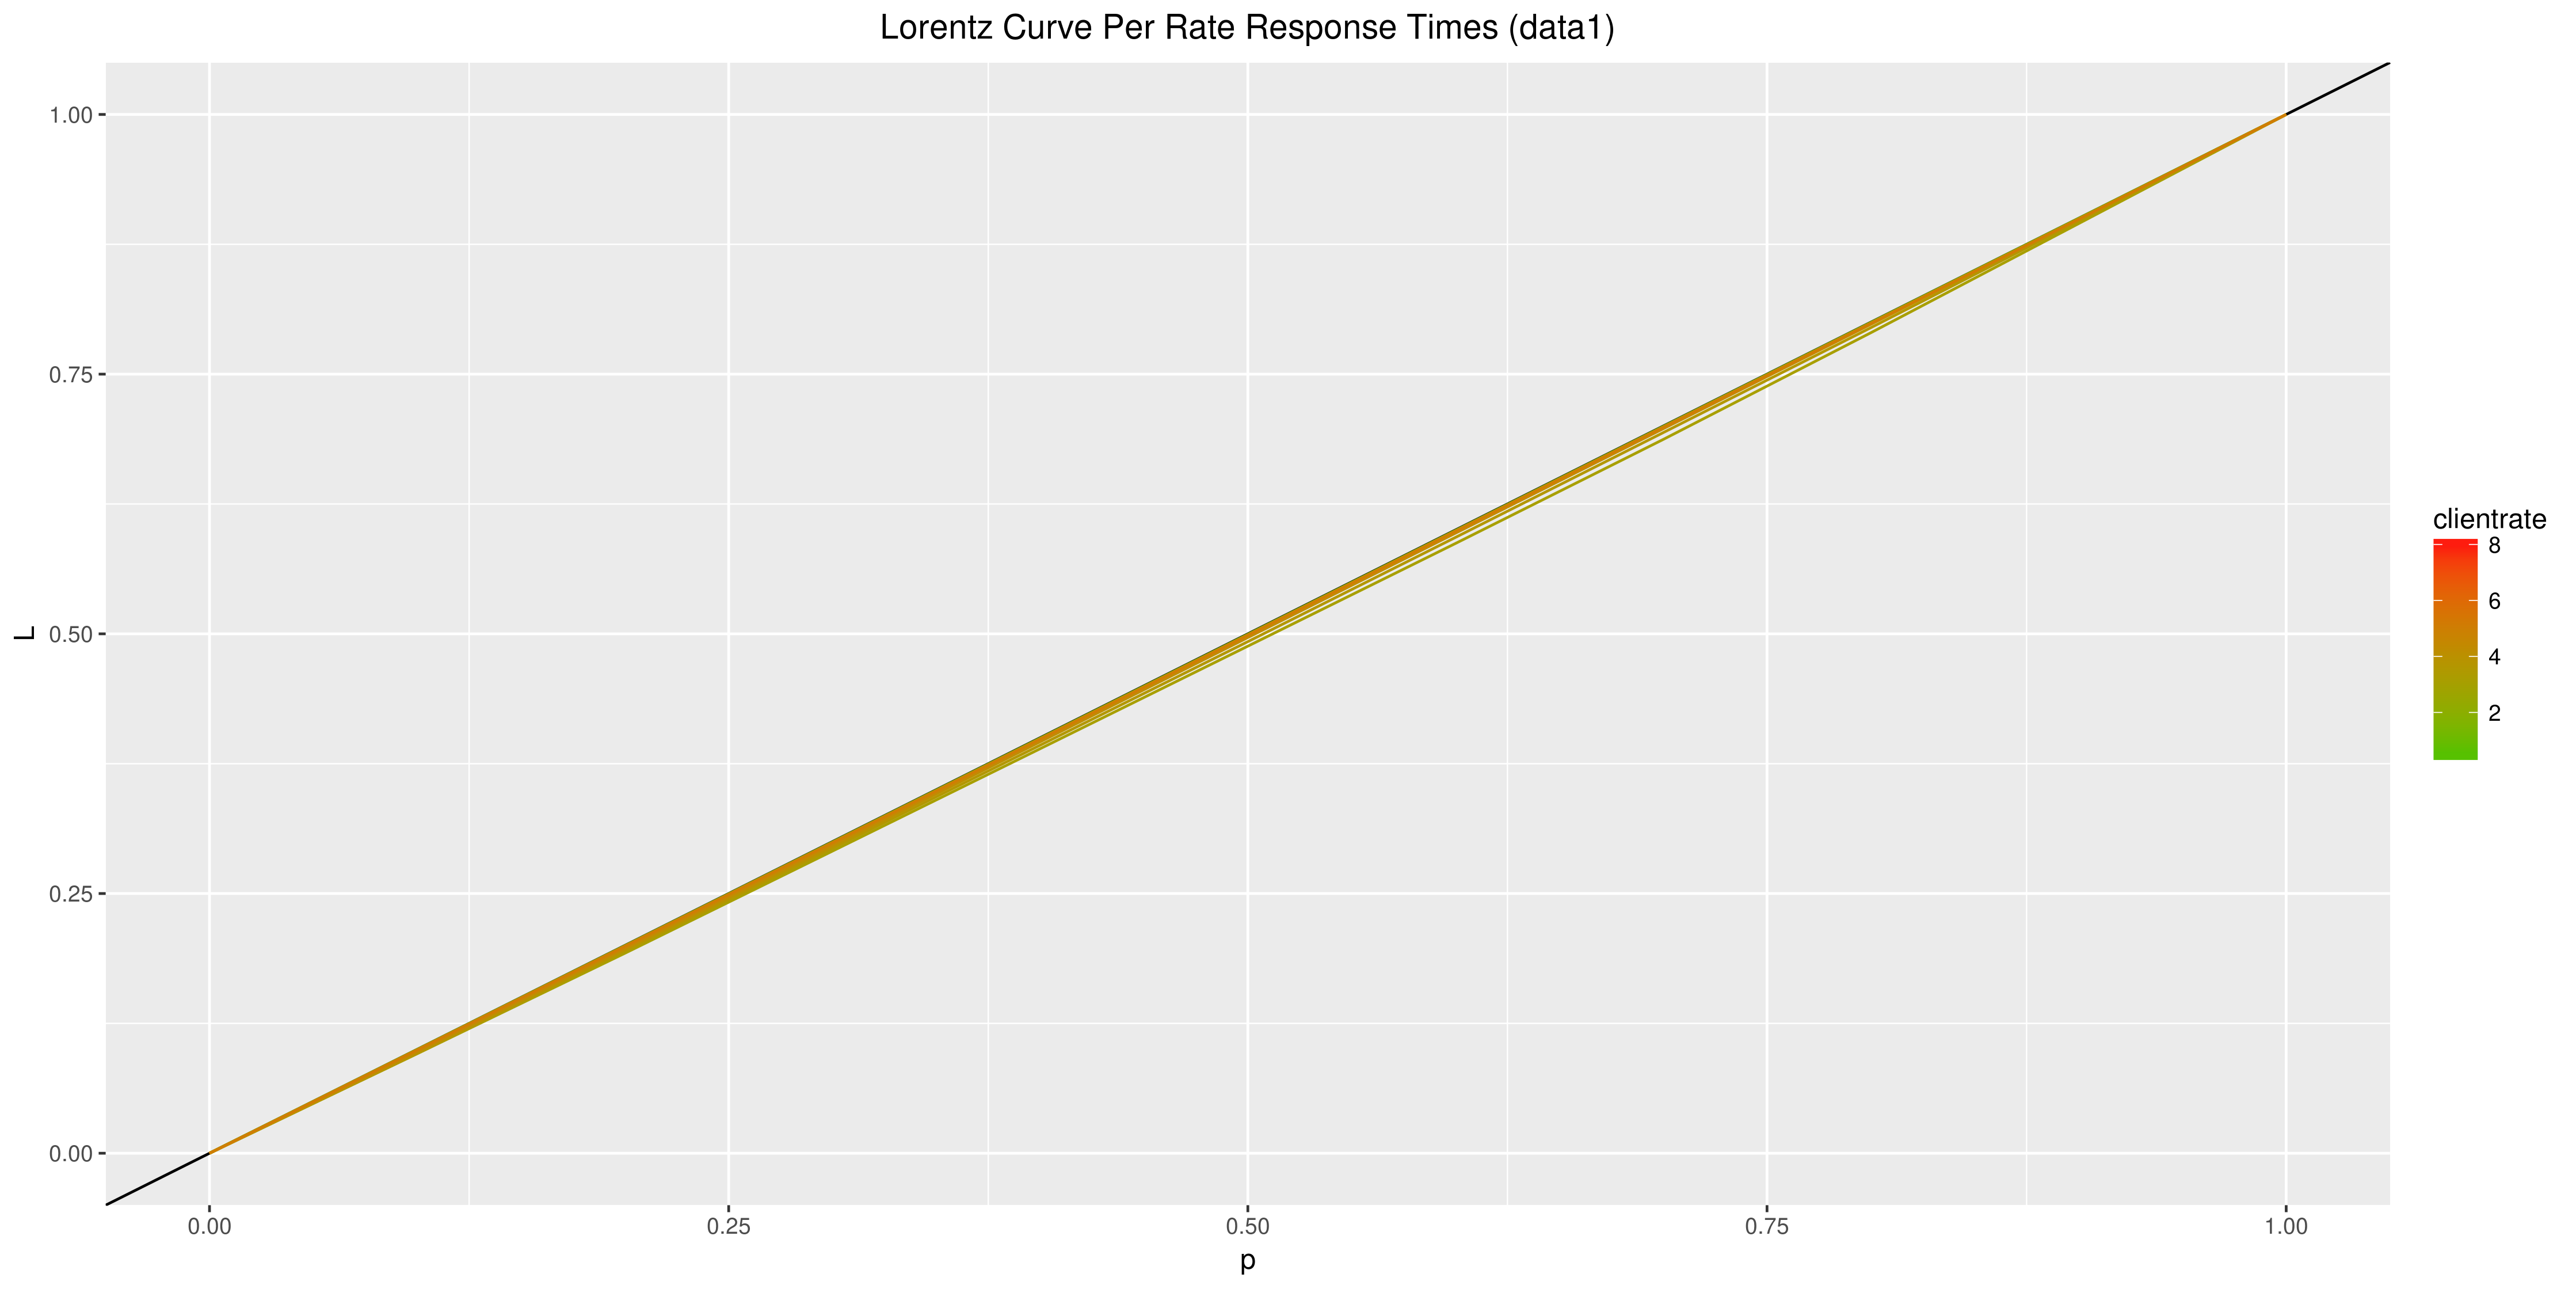
\includegraphics[width=7.5cm]{images/lorenzRT-unifbest}
\end{minipage}
	\caption{Uniform scenario - BestCQI: lorenz curves}
  	\label{fig:Uniform scenario - BestCQI: lorenz curves}
\end{figure}
At the end in order to choose the best scheduler for that scenario we decided to compare the empirical cdf of throughput near the saturation point \(\lambda=3.1\).
\begin{figure}[H]
  \includegraphics[width=1\textwidth]{images/{ecdf-unif-unifbest2.1}.png}
   \caption{Uniform scenario: ECDF comparison \(\lambda=2.1\)}
  \label{fig:Uniform scenario: ECDF comparison lambda2.1}
\end{figure}

\begin{figure}[H]
  \includegraphics[width=1\textwidth]{images/{ecdf-unif-unifbest3.1}.png}
   \caption{Uniform scenario: ECDF comparison \(\lambda=3.1\)}
  \label{fig:Uniform scenario: ECDF comparison lambda3.1}
\end{figure}

We observe that the Best CQI Scheduler is definitely better than the Fair one when \(\lambda \ge \lambda_{sat}\) otherwise the performance are about the same. The fairness is garanted by both scheduler in all \textit{arrival rates} but this is not surprising CQI and service demand have the same uniform distribution for all users. The result is that each users exploits an equal slice of available resources to the antenna. 